\documentclass{article}
\usepackage{amsmath, amssymb, amsfonts}
\usepackage{natbib}
\usepackage{graphicx}
\usepackage{hyperref}
\usepackage{tikz}
\usetikzlibrary{bayesnet}
% ------------------------------------------------------------------------
% Packages
% ------------------------------------------------------------------------
\usepackage{amsmath}

% ------------------------------------------------------------------------
% Macros
% ------------------------------------------------------------------------
%~~~~~~~~~~~~~~~
% List shorthand
%~~~~~~~~~~~~~~~
\newcommand{\BIT}{\begin{itemize}}
\newcommand{\EIT}{\end{itemize}}
\newcommand{\BNUM}{\begin{enumerate}}
\newcommand{\ENUM}{\end{enumerate}}
%~~~~~~~~~~~~~~~
% Text with quads around it
%~~~~~~~~~~~~~~~
\newcommand{\qtext}[1]{\quad\text{#1}\quad}
%~~~~~~~~~~~~~~~
% Shorthand for math formatting
%~~~~~~~~~~~~~~~
\newcommand\mbb[1]{\mathbb{#1}}
\newcommand\mbf[1]{\mathbf{#1}}
\def\mc#1{\mathcal{#1}}
\def\mrm#1{\mathrm{#1}}
%~~~~~~~~~~~~~~~
% Common sets
%~~~~~~~~~~~~~~~
\def\reals{\mathbb{R}} % Real number symbol
\def\integers{\mathbb{Z}} % Integer symbol
\def\rationals{\mathbb{Q}} % Rational numbers
\def\naturals{\mathbb{N}} % Natural numbers
\def\complex{\mathbb{C}} % Complex numbers
\def\simplex{\mathcal{S}} % Simplex
%~~~~~~~~~~~~~~~
% Common functions
%~~~~~~~~~~~~~~~
\renewcommand{\exp}[1]{\operatorname{exp}\left(#1\right)} % Exponential
\def\indic#1{\mbb{I}\left({#1}\right)} % Indicator function
\providecommand{\argmax}{\mathop\mathrm{arg max}} % Defining math symbols
\providecommand{\argmin}{\mathop\mathrm{arg min}}
\providecommand{\arccos}{\mathop\mathrm{arccos}}
\providecommand{\asinh}{\mathop\mathrm{asinh}}
\providecommand{\dom}{\mathop\mathrm{dom}} % Domain
\providecommand{\range}{\mathop\mathrm{range}} % Range
\providecommand{\diag}{\mathop\mathrm{diag}}
\providecommand{\tr}{\mathop\mathrm{tr}}
\providecommand{\abs}{\mathop\mathrm{abs}}
\providecommand{\card}{\mathop\mathrm{card}}
\providecommand{\sign}{\mathop\mathrm{sign}}
\def\rank#1{\mathrm{rank}({#1})}
\def\supp#1{\mathrm{supp}({#1})}
%~~~~~~~~~~~~~~~
% Common probability symbols
%~~~~~~~~~~~~~~~
\def\E{\mathbb{E}} % Expectation symbol
\def\Earg#1{\E\left[{#1}\right]}
\def\Esubarg#1#2{\E_{#1}\left[{#2}\right]}
\def\P{\mathbb{P}} % Probability symbol
\def\Parg#1{\P\left({#1}\right)}
\def\Psubarg#1#2{\P_{#1}\left[{#2}\right]}
\def\Cov{\mrm{Cov}} % Covariance symbol
\def\Covarg#1{\Cov\left[{#1}\right]}
\def\Covsubarg#1#2{\Cov_{#1}\left[{#2}\right]}
\def\Var{\mrm{Var}}
\def\Vararg#1{\Var\left(#1\right)}
\def\Varsubarg#1#2{\Var_{#1}\left(#2\right)}
\newcommand{\family}{\mathcal{P}} % probability family
\newcommand{\eps}{\epsilon}
\def\absarg#1{\left|#1\right|}
\def\msarg#1{\left(#1\right)^{2}}
\def\logarg#1{\log\left(#1\right)}
%~~~~~~~~~~~~~~~
% Distributions
%~~~~~~~~~~~~~~~
\def\Gsn{\mathcal{N}}
\def\Ber{\textnormal{Ber}}
\def\Bin{\textnormal{Bin}}
\def\Unif{\textnormal{Unif}}
\def\Mult{\textnormal{Mult}}
\def\Cat{\textnormal{Cat}}
\def\Gam{\textnormal{Gam}}
\def\InvGam{\textnormal{InvGam}}
\def\NegMult{\textnormal{NegMult}}
\def\Dir{\textnormal{Dir}}
\def\Lap{\textnormal{Laplace}}
\def\Bet{\textnormal{Beta}}
\def\Poi{\textnormal{Poi}}
\def\HypGeo{\textnormal{HypGeo}}
\def\GEM{\textnormal{GEM}}
\def\BP{\textnormal{BP}}
\def\DP{\textnormal{DP}}
\def\BeP{\textnormal{BeP}}
%~~~~~~~~~~~~~~~
% Theorem-like environments
%~~~~~~~~~~~~~~~

%-----------------------
% Probability sets
%-----------------------
\newcommand{\X}{\mathcal{X}}
\newcommand{\Y}{\mathcal{Y}}
\newcommand{\D}{\mathcal{D}}
\newcommand{\Scal}{\mathcal{S}}
%-----------------------
% vector notation
%-----------------------
\newcommand{\bx}{\mathbf{x}}
\newcommand{\by}{\mathbf{y}}
\newcommand{\bt}{\mathbf{t}}
\newcommand{\xbar}{\overline{x}}
\newcommand{\Xbar}{\overline{X}}
\newcommand{\tolaw}{\xrightarrow{\mathcal{L}}}
\newcommand{\toprob}{\xrightarrow{\mathbb{P}}}
\newcommand{\laweq}{\overset{\mathcal{L}}{=}}
\newcommand{\F}{\mathcal{F}}


\title{Inference of Dynamic Regimes in the Microbiome}
\author{Kris Sankaran}
\begin{document}
\maketitle

A typical microbiome data set describes the abundances of bacterial species
across samples. To this point, we have studied latent structure across species
and samples separately. For example, we have developed interactive visualization
techniques to compare subsets of species, and we have applied mixed-membership
models to characterize variation in samples across timepoints. In contrast, our
goal here is to study latent structure across species and samples
simultaneously. This difference is analogous to the change in perspective
obtained by studying a coclustering rather than two separate clusterings, or an
ordination biplot instead of simply the scores or loadings. We will focus on the
case where samples are collected over time, so that this problem can be
understood as one of detecting dynamic regimes, as explained in section
\ref{sec:problem_description}

The primary contributions of this chapter are,
\begin{itemize}
\item The relation of the regime detection problem to several statistical
  frameworks, and a comparison of the types of interpretation facilitated by
  each.
\item Developing experiments to evaluate the practical utility of these
  different formulations.
\item A catalog of algorithm pseudocode and real implementations, to serve as a
  reference for researchers interested in regime detection.
\item The design of and code for static visualizations that can be used to
  evaluate the results of various methods.
\end{itemize}

In section \ref{sec:problem_description}, we describe the scientific problem of
interest in more detail and provide a high-level statistic formulation. In
section \ref{sec:baseline}, we describe approaches which are easy to implement,
but that fail to incorporate temporal structure -- these serve as reference
points for evaluating more complex models.
Sections \label{sec:temporal_probabilistic_models}
and \label{sec:temporal_mixture_models} review and apply smoothing and mixture
modeling techniques to this problem, while
section \label{sec:alternative_probabilistic_models} highlights several
departures of typical microbiome data from the structure assumed by the
techniques in previous sections, along with references to literature that
addresses these departures.

\section{Problem description}
\label{sec:problem_description}

In latent variable modeling, our ultimate goal is a succint representation of
complex data. In a way, we can think of the reduced representations as a type of
data compression for human interpretation, and as in any (lossy) compression,
there is a choice of what structure to preserve. Different reduced
representations facilitate different comparisons -- for example, clustering
bacteria allows easy comparison of taxonomic categories, while clustering
samples allows a comparison of full community states.

In the regime detection problem, the comparisons we would like to facilitate are
\begin{itemize}
\item For each species, can we assign time intervals to different dynamic
  regimes?
\item Can we define subsets of species which have similar patterns of behavior,
  in terms of these regimes?
\end{itemize}

Conceretely, we may expect that over the time course of a study, individual
species may switch between stable / unstable, increasing / decreasing, or
present / absent regimes, either due to natural ecological dynamics or
experimentally induced perturbations. We would like to detect these alternative
regimes automatically.

Further, as we are typically working with hundreds or thousands of bacterial
species at a time, we would like to group or relate species according to these
regimes, so that (1) we do not need to inspect the regime switching for
individual species one by one (2) we can achieve gains in power by pooling
across species. The resulting species groups can be related to available taxonomic
information to draw scientific conclusions about the behavior of different
taxa during different sampling periods -- for example, ``70\ of the Bacteroides
exhibited stability during the first half of the antibiotic time course, while
the rest showed decreasing trends.''

We can frame this analysis problem using the language of latent variables. Let
$\left(t_{i}\right)_{i = 1}^{n}$ be the sampling timepoints, and index species by
$\left(s_{j}\right)_{j = 1}^{p}$. Our goal is to infer a function $\theta$
mapping time by species pairs $\left(t_{i}, s_{j}\right)$ to an associated
latent state, which can either belong to a discrete set of $K$ types,
$theta\left(t_{i}, s_{j}\right) \in \{1, \dots, K\}$, or which might described a
mixed-memberhip, $\theta\left(t_{i}, s_{j}\right) \in \S^{K - 1}$, where
$\S^{K - 1}$ is the $K - 1$-dimensional simplex.

We expect the function $\theta$ to be reasonably well-behaved over time.
Further, by comparing $\theta\left(\cdot, s_{j}\right)$ across different species
$j$, we can group or sort species according to their regime membership behavior.
See Figures \ref{fig:partition} and \ref{fig:gradient} for visual explanations
of this analysis approach.

\section{Methods baseline}
\label{sec:baseline}

\subsection{Hierarchical Clustering}

As a baseline, we create a heatmap as in Figure \ref{fig:partition}, where
species are ordered according to a hierarchical clustering tree. Note that
clustering trees are invariant under left-right swaps of branches; to fix a
unique tree, we order branches so that the average abundance of the left is
always larger than those on the right. The resulting ordered heatmap could
potentially resolve partitions in the species by time space. A limitation of
this approach is that it does not provide any clustering for the timepoints,
only species, even if blocks across timepoints seem to appear in the resulting
heatmap. Coclustering species and timepoints is not a sufficient alternative,
because the blocking across timepoints must respect the known order. Conversely,
an advantage of this approach is that it is simple to both implement this method
and interpret the results.

The figure generated by hierarchical clustering will be sensitive to several
choices,
\begin{itemize}
\item Transformations: Different transformations might be more effective
  representations of the underlying data.
\item Distance: Different distances are appropriate for different types of data.
\end{itemize}

For example, some natural transformations are
\begin{itemize}
\item $\asinh$-transformed: Raw count data in microbiome data sets tend to
  be very heavy tailed, but with a large spike at 0. An $\asinh$-transformation
  behaves like $\log$-transformation for large counts, but goes through the
  origin -- this downweights coordinates with large counts. This can be seen
  from the representation $\asinh\left(x\right) = \logarg{(x + \sqrt{1 -
      x^{2}}}$.
\item Innovations: Rather than clustering the raw series, we can cluster the
  differenced series. This will cluster series that have similar changes between
  neighboring timepoints, even if their overall values are quite different. This
  can highlight bacterial series with similar dynamics, at the cost of failing
  to resolve changes resulting from different overall abundances.
\item Binarized: We can transform the series $x_{i}$ into $\indic{x_{i} > 0}$.
  This loses substantial information, but measuring differences in presence /
  absence patterns in microbiome studies can be scientifically meaningful.
\end{itemize}

On these transformed data, we now need to compute pairwise distances between
series. Three choices that we consider are,
\begin{itemize}
\item Euclidean: This distance is ideal when clusters have a spherical shape in
  a high-dimensional space.
\item Jaccard: This is a distance between pairs of length $p$ binary sequences
  $x_{i}$ and $x_{j}$ defined as
\begin{align}
  d\left(x_{i}, x_{j}\right) &= 1 - \frac{\sum_{k = 1}^{p} \indic{x_{ik} = x_{jk} = 1}}{p},
\end{align}
or one minus the fraction of coordinates that are 0/1. The motivation for this
distance is that coordinates that are both 0 should not contribute to similarity
between sequences, especially when they may be dominated by 0s. We apply this
distance to the binarized version of the species counts.
\item Mixture: Since any convex combination of distances is still a distance, we
  can define mixtures of distances that reflect several characteristics of the
  data.
\end{itemize}

In general, we have no quantitative approach for comparing the clusterings
obtained by different distances. Instead, we compare the resulting heatmaps,
noting how different patterns are identified by different approaches.

An example application to the $\asinh$-transformed antibiotics data is provided
in Figures \ref{} through \ref{}. Recall that this data set tracks the abundance
of bacterial species over three subjects across several months, including two
brief antibiotic treatment regimes -- see section
\ref{subsec:bacterial-dynamics-of-antibiotics-time-courses} for further details.


The heatmaps in Figures \ref{fig:heatmap-euclidean} through
\ref{fig:heatmap-innovations-bin} describe which species have simialr behaviors.
The three main column panels correspond to the three study subjects. Each row
gives the time series of abundances for a single species, with time evolving
from left to right and abundance indicated by heatmap shade intensity. The
taxonomic identities of these species is provided by the multicolored bar on the
left. The rowwise panels correspond to different subtrees of the hierachical
clustering when choosing to cut at a particular height -- note that the clusters
tend to have highly imbalanced sizes. The most important takeaways from these
figures are that they show which groups of bacteria are most strongly affected
by the antibiotic treatment, as well as how long they take to recover.

\begin{figure}[ht]
  \centering
  %\includegraphics[width=0.8\textwidth]{figure/heatmap-euclidean}
  \caption{\label{fig:heatmap-euclidean} }
\end{figure}

\begin{figure}[ht]
  \centering
  %\includegraphics[width=0.8\textwidth]{figure/heatmap-jaccard}
  \caption{\label{fig:heatmap-jaccard} }
\end{figure}

\begin{figure}[ht]
  \centering
  %\includegraphics[width=0.8\textwidth]{figure/heatmap-mix}
  \caption{\label{fig:heatmap-mix} }
\end{figure}

\begin{figure}[ht]
  \centering
  %\includegraphics[width=0.8\textwidth]{figure/heatmap-innovations}
  \caption{\label{fig:heatmap-innovations} }
\end{figure}

\begin{figure}[ht]
  \centering
  %\includegraphics[width=0.8\textwidth]{figure/heatmap-innovations-bin}
  \caption{\label{fig:heatmap-innovations-bin} }
\end{figure}

As expected, different distances group series according to the features that
define the distance. For example, the Jaccard distance groups series with
similar zero patterns, even if their associated abundances are very different.
On the other hand, the euclidean distance tends to group series with similar
averages, and there is less blocking by presence-absence structure. Notice that,
according to the colored bar indicating taxonomic identity, families are not
scattered randomly across rows, but they are not separated into completely
disjoint blocks either. This suggests that while phylogenetic identity certainly
relates to the patterns of abundance over time course, variation is occuring at
levels of granularity more subtle than family level.

To summarize the behavior within clusters, we display the centroids in Figures
\ref{fig:centroid-euclidean-conditional} through
\ref{fig:centroid-mix-presence}. The panel number indicates the cluster as
defined by cutting hierarchical clustering, with the same labeling as in the
heatmap. Different individuals are represented by different colors. The solid
points are time series of averages across all species for the given cluster, for
the current individual. The semitransparent points are the raw values used to
compute these averages. Evidently, some of the clustering structure is due
simply to the presence of species within only some of the patients. Further,
differential responses can be seen within some of the panels. For example,
cluster 17 includes bacteria that are affected by the first antibiotics time
course, but only for patients D and F, and which are also only affected in
subject D during the second time course.

The fact that the data include many zeros makes computing averages groups a
somewhat misleading cluster summary. Instead, we can decompose the summary into
a presence-absence component and a value-conditional-on-presence component.
The presence-absence component computes the proportion of bacteria that are
present at any given timepoint, while the conditional-positive component
computes the time averages among all observed bacteria.

\begin{figure}[ht]
  \centering
  %\includegraphics[width=0.9\textwidth]{figure/centroid-euclidean-conditional}
  \caption{\label{fig:centroid-euclidean-conditional} }
\end{figure}

\begin{figure}[ht]
  \centering
  %\includegraphics[width=0.9\textwidth]{figure/centroid-euclidean-presence}
  \caption{\label{fig:centroid-euclidean-presence} }
\end{figure}

\begin{figure}[ht]
  \centering
  %\includegraphics[width=0.9\textwidth]{figure/centroid-innovations-conditional}
  \caption{\label{fig:centroid-innovations-conditional}}
\end{figure}

\begin{figure}[ht]
  \centering
  %\includegraphics[width=0.9\textwidth]{figure/centroid-innovations-presence}
  \caption{\label{fig:centroid-innovations-presence}}
\end{figure}

\begin{figure}[ht]
  \centering
  %\includegraphics[width=0.9\textwidth]{figure/centroid-jaccard-conditional}
  \caption{\label{fig:centroid-jaccard-conditional}}
\end{figure}

\begin{figure}[ht]
  \centering
  %\includegraphics[width=0.9\textwidth]{figure/centroid-jaccard-presence}
  \caption{\label{fig:centroid-jaccard-presence}}
\end{figure}

\begin{figure}[ht]
  \centering
  %\includegraphics[width=0.9\textwidth]{figure/centroid-mix-conditional}
  \caption{\label{fig:centroid-mix-conditional}}
\end{figure}

\begin{figure}[ht]
  \centering
  %\includegraphics[width=0.9\textwidth]{figure/centroid-mix-presence}
  \caption{\label{fig:centroid-mix-presence}}
\end{figure}

\subsection{CART}

While placing similar time series near to one another suggests time windows
where the series behave similarly to one another, the hierarchical clustering
approach presented above does not explicitly partition timepoints into windows
with distinct behaviors. In this section, we consider a slight extension that
provides such a partitioning.

The main idea is that a regression tree that uses $X$ to predict $y$ provides a
partition of the $X$ space, where $y$ has lower variation within than between
partitions \citep{breiman1984classification}. We will the hierarchical
clustering approach from the previous section to obtain an ordering $s_{j} \in
\{1, \dots, n_{\text{species}}\}$ across species. We write the timepoint for the
$i^{th}$ sample as $t_{i}$ Then, we model the count for the $j^{th}$ species in
the $i^{th}$ sample as $y_{ij} \approx f\left(s_{j}, t_{i}\right)$ using
$f \in \mathcal{T}$ the space of decision trees. The output of interest is the
fitted partition on $\left(s_{j}, t_{i}\right)$.

\subsubsection{CART review}
\label{subsubsec:cart_review}

For completeness, we review the CART algorithm. Following \citep{stat315bnotes},
we can describe it in terms of (1) the structural model, (2) the score criterion
for choosing between models, and (3) the search strategy used to produce the
final fit.

The structural model $\mathcal{F}$ is the class of functions that can be
expressed as
\begin{align}
f\left(x\right) &= \sum_{m = 1}^{M} c_{m} \indic{x \in R_{m}},
\end{align}
where $\left(R_{m}\right)_{m = 1}^{M}$ are some partition of the covariate space
and $c_{m} \in \reals$ are constants associated with each partition element.

For regression, the criterion is the expected generalization squared-error
between $y_{i}$ and the $c_{m}$ associated with the $R_{m}$ within which the
covariate $x_{i}$ lies -- we will denote this by $c\left(x_{i}\right)$. In
classification, the corresponding criterion is the expected missclassification
error. More precisely, we consider the empirical risks
\begin{align}
  \frac{1}{n} \sum_{i = 1}^{n} \left(y_{i} - c\left(x_{i}\right)\right)^{2},
\end{align}

for regression and
\begin{align}
  \frac{1}{n} \sum_{i = 1}^{n} L_{y_{i}, c\left(x_{i}\right)} \indic{y_{i} = c\left(x_{i}\right)},
\end{align}
for classification, where $L_{kk^{\prime}}$ is the loss induced by
missclassifying $k$ as $k^{\prime}$. Since the empirical risk on the training
data underestimates generalization error, these estimates are constructed on
test sets.

To obtain a fitted $\hat{f} \in \mathcal{F}$, the algorithm must identify a
partition $\left(R_{m}\right)$ and constants $c_{m}$ (approximately) minimizing
the score criterion. Given a particular $R_{m}$, fitting $c_{m}$ is
straightforwards, since the score decouples across partition elements -- in the
regression case the minimizers are averages of the $y_{i}$s or majority votes
within partition elements. On the other hand, finding the optimal $R_{m}$ is an
intractable combinatorial optimization problem, and the search strategy instead
uses a greedy approach to obtain a reasonable local minimizer.

More precisely, the final partition is found by recursively splitting the
input space, and then pruning away splits that seem less relevant. At the first
step, the partition consists of a single $R_{1}$, equal to the entire covariate
space, and it is split on covariate $j^{\ast}$ at position $t_{j1}^{\ast}$
that solve the optimization
\begin{align}
  \left(j^{\ast}, t_{j1}^{\ast}\right) &= \arg \min_{\substack{j = 1, \dots, p \\ t_{j1} \in \reals}} \sum_{i \in R_{1, l}} \left(y_{i} - \bar{y}_{l}\right)^{2} + \sum_{i \in R_{1, r}} \left(y_{i} - \bar{y}_{r}\right)^{2}
\end{align}
where $R_{1, l}$ and $R_{1, r}$ (for ``left'' and ``right'') are a splitting of
$R_{1}$ along feature $j$ feature at position $t_{j1}$.

This procedure is iterated recursively. That is, at the $m^{th}$ iteration, the
next split solves nearly the same optimization,
\begin{align}
  \left(m^{\ast}, j^{\ast}, t_{jm}^{\ast}\right) &= \arg \min_{\substack{j = 1, \dots, p \\ t_{jm} \in \reals}} \sum_{i \in R_{m, l}} \left(y_{i} - \bar{y}_{l}\right)^{2} + \sum_{i \in R_{m, r}} \left(y_{i} - \bar{y}_{r}\right)^{2},
\end{align}
where the main difference is that we must now choose which of the $m$ previously
defined partition elements to split.

This is done for some prespecified number of splits, $M$. This partition is
potentially unecessarily highly resolved, and it can improve generalization
error to introduce a pruning step. Define $C_{m}$ denote the ``cost'' of a
(potentially intermediate) partition element $R_{m}$ according to,

\begin{align}
  C_{m} &= \begin{cases}
    \hat{r}_{m} + k & \text{if $m$ was never split} \\
    \sum_{m^\prime} C_{m^{\prime}} & \text{if $m$ was split into two $m^{\prime}$}
    \end{cases}
\end{align}
where $\hat{r}_{m} = \sum_{x_{i} \in R_{m}} \left(y_{i} - c_{m}\right)^{2}$. $k$
can be interpreted as the amount of improvement to the score criterion that the
split must provide in order to be accepted. The
final partitioning is obtained by choosing to split or merge each intermediate
$m$ so that $C_{m}$ is minimized. Specifically, if
$\hat{r}_{m} + k < \sum_{m^{\prime}} C_{m^{\prime}}$, then all descendant nodes
(subpartition elements) are merged into $R_{m}$. Otherwise, the left and right
splits are accepted. These choices are made sequentially, from the bottom up.

\subsubsection{Antibiotics application}
\label{subsubsec:antibiotics_application}

An example of the type of output generated by this approach is provided in
Figure \ref{fig:rpart_complex}. As in the heatmaps produced by hierarchical
clustering, the three vertical panels represent three subjects, while rows and
columns correspond to species and temporally-ordered samples, respectively. The
rows have been ordered according to a hierarchical clustering on the mixed
Euclidean + Jaccard distance described above. The shading within partition
blocks corresponds to the fitted $\hat{c}_{m}$ from the regression tree.

Note the presence of two dark vertical stripes in subjects D and F -- these
correspond to the two antibiotic treatment regimes. In general, ``wide'' blocks
are more common than ``tall'' ones. This reflects the fact that timepoints
within bacteria tend to have more similar abundances, compared to multiple
bacteria at a single timepoint, even when those bacteria have been ordered by a
overall hierarchical clustering.

One interesting detail is the delayed, or sometimes nonexistent, recovery after
the first antibiotic time course among a cluster of bacteria near the bottom of
the panel for subject F. This long-term impact of antibiotics on bacterial
populations, at least in one patient, was a central finding in
\citep{dethlefsen2011incomplete}. Observe that a similar pattern is visible after
the second antibiotic time course among patient D, also for species near the
bottom of the panel.

Related views are given in Figures \ref{fig:rpart_simple} through
\ref{fig:rpart_conditional}. Figures \ref {fig:rpart_simple} through
\ref{rpart_complex_3} give analogous fits for different complexity parameters
$k$. Figures \ref{fig:rpart_binary_simple} and \ref{fig:rpart_conditional}
decompose the prediction problem into just a binary part and a
conditional-on-positivity part, using the hurdle heuristic.

Two limitations become clear in this example application. First, partitioning
across species seems hard to obtain simultaneously across all subjects -- in
Figure \ref{fig:rpart_complex}, there seem to be no ``tall'' blocks for Subject
E. This is a consequence of first ordering all species according to a
hierarchical clustering based on all subjects. A potential solution would be to
cluster the species separately across subjects, trading off the ability to match
the same species across several panels in order to better study species blocking
within subjects.

Second, these global views of the data make it difficult to inspect individual
species and sample identities. Potential solutions are (1) link necessary
supplemental (e.g., taxonomic) information within the static view, through a
shaded taxonomic-family stripe, for example, or (2) construct an interactive
version of these plots, where hovering over a partition element provides focused
information about that element (e.g., the species identities it contains), in
the spirit of our \texttt{hclustvis} package.

\begin{figure}[ht]
  \centering
  \includegraphics[width=0.8\textwidth]{figure/rpart_complex}
  \caption{\label{fig:rpart_complex} }
\end{figure}

\section{Temporal probabilistic models}
\label{sec:temporal_probabilistic_models}

In section \ref{sec:baseline}, we described distance and regression-based
techniques to approaching the questions outlined in
\ref{sec:problem_description} of identifying which subsets of species have
similar abundance profiles during which windows of time. In particular, we have
avoided any direct modeling of abundances across species or over time. From this
point onwards, we adopt this alternative approach, using the approaches of
\ref{sec:baseline} as a reference for what analysis is possible with minimal
effort.

In this section, we first review two fundamental approaches to probabilistic
temporal modeling which are used as building blocks in section
\ref{sec:temporal_mixture_models}: linear dynamical systems (section
\ref{subsec:linear_dynamical_systems}) and gaussian processes (section
\ref{subsec:gaussian_processes}). These approaches are designed for single time
series, or collections of independent ones. However, models that consider
collections of related time series can be constructed from these, by introducing
latent variables.

\subsection{Gaussian Processes}
\label{subsec:gaussian_processes}

Gaussian Processes (GPs) provide a prior over classes of stationary, smoothly
varying functions. Their appeal as a probabilistic modeling building block lies
in the fact that they are simultaneously nonparametric -- they can adapt to more
complex functions as more data arrives -- while still admitting tractable
inference. One of the simplest models involving GPs models observations
$\left(x_{i}, y_{i}\right) \in \reals^{p}\times R$ as

\begin{align}
y_{i} &= f\left(x_{i}\right) + \eps_{i}
\end{align}

where $f \sim GP\left(m, \kappa\right)$, meaning that for any collections of
covariates $\left(x_{1}, \dots, x_{n}\right)$, we have

\begin{align}
  \left(f\left(x_{1}\right), \dots, f\left(x_{n}\right)\right) &\sim
  \Gsn\left( \begin{pmatrix} m\left(x_{1}\right) \\ \vdots \\ m\left(x_{n}\right) \end{pmatrix}, \begin{pmatrix} \kappa\left(x_{1}, x_{1}\right) & \dots & \kappa\left(x_{1}, x_{n}\right) \\ \vdots & & \vdots \\ \kappa\left(x_{n}, x_{1}\right) & \dots &\kappa\left(x_{n}, x_{n}\right) \end{pmatrix}\right)
\end{align}
$m$ and $\kappa$ are called the mean and covariance functions, respectively. We
will denote this covariance matrix of $\kappa$'s applied to pairs of $x_{i}$ by
$K\left(x, x\right)$.

It is common to initially center the data before analysis, in which case we can
assume $m \equiv 0$. Further, any positive-definite covariance function $\kappa$
can be used -- a common choice is the Gaussian covariance,

\begin{align}
\kappa_{\sigma_{f}, M}\left(x_{p}, x_{q}\right) &= \sigma_{f}^{2}\exp{-\frac{1}{2}\left(x_{p} - x_{q}\right)^{T}M\left(x_{p} - x_{q}\right)},
\end{align}

where $M$ can be $\frac{1}{l^{2}}I_{n}$, which assumes similar degrees of smoothness
across all coordinates, $\diag\left(l\right)^{-2}$, which allows different
smoothness along different axes, or $\Lambda \Lambda^{T} + \diag\left(l\right)^{-2}$,
which assumes variation along certain non-axes-aligned directions. While a
reasonable defult, it is good practice to adapt the covariance function to the
data problem at hand, accounting for seasonality, multiple scales of variation,
or the presence of outliers, see section 5.4.3 of \citep{rasmussen2006gaussian}
for an in depth example. Note that the covariance function is responsible for
the GPs emphasis on smooth trajectories rather than transient events. However,
multiscale behavior can be modeled by introducing mixtures, as we will see in
section \ref{sec:temporal_mixture_models}.

A plate diagram representing this model is provided in Figure \ref{fig:gp_plate}.

\begin{figure}[ht]
  \centering
  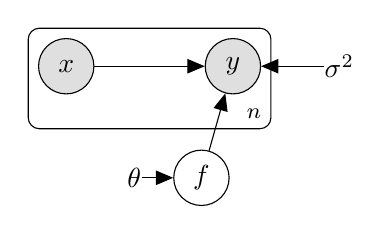
\begin{tikzpicture}
    \node[obs] (y) {$y$};
    \node[latent, below=0.7 of y, xshift=-0.4cm] (f) {$f$};
    \node[obs, left=of y, xshift=-0.4cm]  (x) {$x$};
    \node[const, right=of y, xshift=-0.2cm]  (sigma) {$\sigma^2$};
    \node[const, left=0.4 of f] (theta) {$\theta$};

    % Connect the nodes
    \edge {x, f, sigma} {y} ; %
    \edge {theta} {f} ; %

    % Plates
    \plate {yx} {(x)(y)} {$n$} ;
  \end{tikzpicture}

  \caption{Gaussian Process plate diagram.\label{fig:gp_plate} }
\end{figure}


In this model, the posterior of $f$ is available analytically, by virtue of
Gaussian-Gaussian conjugacy. Consider evaluating the function $f$ at new points
$x_{\ast}$, denoted by $f_{\ast} := f\left(x_{\ast}\right)$. Then, the joint of
$y$ and $f^{\ast}$ is
\begin{align}
  \begin{pmatrix}
    y \\ f_{\ast}
  \end{pmatrix} &= \Gsn\left(
 \begin{pmatrix}
   0 \\ 0
 \end{pmatrix} ,
\begin{pmatrix}
  K\left(x, x\right) + \sigma^{2}I_{n} & K\left(x, x_{\ast}\right) \\
  K\left(x_{\ast}, x\right) & K\left(x_{\ast}, x_{\ast}\right)
\end{pmatrix}
  \right),
\end{align}
which yields the posterior,
\begin{align}
  f_{\ast} \vert y &\sim \Gsn\left(\Earg{f_{\ast} \vert y}, \Covarg{f_{\ast} \vert y}\right),
\end{align}
where
\begin{align}
  \Earg{f_{\ast} \vert y} &= K\left(x_{\ast}, x\right)\left(K\left(x, x\right) + \sigma^{2}I_{n}\right)^{-1}y \\
  \Covarg{f_{\ast} \vert y} &= K\left(x_{\ast}, x_{\ast}\right) - K\left(x_{\ast}, x\right)\left(K\left(x, x\right) + \sigma^{2}I_{n}\right)^{-1}K\left(x, x_{\ast}\right)
\end{align}
Note the $n\times n$ matrix inversion in the covariance calculation. This is the
source of the $O\left(n^{3}\right)$ complexity of using standard GPs, though a
variety of fast approximations have been proposed, exploiting the sparse,
banded, or block structure within the covariance
\citep{quinonero2007approximation}.

In this computation, we have assumed the the kernel hyperparameters $\theta$ is
known\footnote{For example, in the Gaussian covariance case, this has the form
  $\theta = \left(\sigma_{f}^{2}, M\right)$}. In reality, these must be inferred
from the data. Two standard approaches are based on maximizing (1) the marginal
likelihood of $y$ and (2) the cross-validated predictive likelihood. The first
approach leverages the fact that the marginal likelihood,
\begin{align}
\log p\left(y \vert x; \theta\right) &= -\frac{n}{2}\log 2\pi - \log\absarg{K_{\theta}\left(x, x\right) + \sigma^{2}I_{n}} - \frac{1}{2}y^{T}\left(K_{\theta}\left(x, x\right) + \sigma^{2}I_{n}\right)^{-1}y
\end{align}
and its gradients over $\theta$ have a closed form, and so can be optimized.

The cross-validation approach instead maximizes the average predicted log probability,
\begin{align}
\sum_{i = 1}^{n} \log p\left(y_{i} \vert x, y_{-i}; \theta\right),
\end{align}
which can also be found analytically, by conditioning the marginal for $y$.

- Review GP graphical model
- Basic distinctions from previous models
- Description of GP posterior
  + GP pseudocode
  + Link to some actual code

\subsection{Linear dynamical systems}
\label{subsec:linear_dynamical_systems}

Linear dynamical systems model an observed time series as a transformation of
temporally evolving latent states. The basic idea reminds me of trying to swat a
fly. I might hear a buzzing noise, which gives some sense of where the fly is,
and I might know that it can't move too far too quickly, but I might only get a
few brief glimpses of the actual insect. The evolving latent state here is the
true position of the fly, while the transformation that we observe is the
loudness of the buzzing. There have been many proposals that allow general
transformation and state evolution behavior, but a fundamental starting point is
the linear-gaussian dynamical system,

\begin{align}
  z_{t} &= A z_{t - 1} + w_{t} \\
  x_{t} &= C z_{t} + \eps_{t} \\
  w_{t} &\sim \Gsn\left(0, \Lambda\right) \\
  \eps_{t} &\sim \Gsn\left(0, \Sigma\right).
\end{align}

The $z_{t}$'s are a markov chain of latent states, while the $x_{t}$'s represent
the observed emissions from it. $A$ and $\Lambda$ govern the dynamics of the
underlying process, while $C$ and $\Sigma$ describe the emission structure. The
associated graphical model is provided in Figure \ref{fig:lds_graphical}.

There are two conceptual components to fitting this model,

\begin{itemize}
\item Inference: Even if $\Theta = \{A, C, \Lambda, \Sigma\}$ were known, there
  is often value in estimating the latent $z_{i}$.
\item Learning: Typically, the parameters $\Theta$ are unknown, and must
  themselves be learned from the data.
\end{itemize}

Further, inference can be approached in several different ways, depending on
problem context and constraints. Among the most common approaches are

\begin{itemize}
\item Filtering: Update beliefs of the current latent state in an online
  fashion. Quantitatively, the goal is to estimate the distribution
  $p\left(z_{t} \vert x_{1:t}\right)$.
\item Smoothing: Use the full history to estimate beliefs of each latent state,
  one at a time. This means to estimate $p\left(z_{t} \vert x_{1:T}\right)$ for
  each $t = 1, \dots, T$.
\item Forecasting: Predict the next few latent states given all observations so
  far. For example, we might be interested in $p\left(z_{t + 1} \vert
  x_{1:t}\right)$.
\end{itemize}

\begin{figure}[ht]
  \centering
  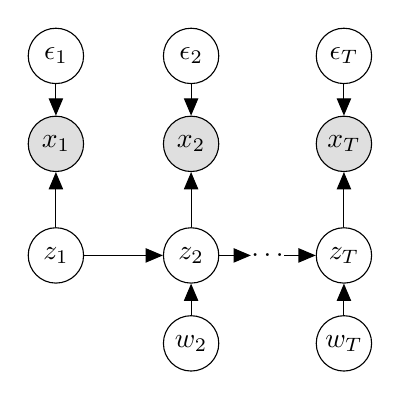
\begin{tikzpicture}
    \node[obs] (x1) {$x_{1}$};
    \node[latent, above=0.4 of x1] (eps1) {$\eps_{1}$};
    \node[latent, below=0.7 of x1] (z1) {$z_{1}$};
    \node[obs, right=of x1] (x2) {$x_{2}$};
    \node[latent, above=0.4 of x2] (eps2) {$\eps_{2}$};
    \node[latent, right=of z1] (z2) {$z_{2}$};
    \node[latent, below=0.4 of z2] (w2) {$w_{2}$};
    \node[const, right=0.4 of z2] (zdots) {$\ldots$};
    \node[latent, right=0.4 of zdots] (zT) {$z_{T}$};
    \node[latent, below=0.4 of zT] (wT) {$w_{T}$};
    \node[obs, above=0.7 of zT] (xT) {$x_{T}$};
    \node[latent, above=0.4 of xT] (epsT) {$\eps_{T}$};
    
    % Connect the nodes
    \edge {z1} {x1} ; %
    \edge {z2} {x2} ; %
    \edge {z1} {z2} ; %
    \edge {z2} {zdots} ; %
    \edge {zdots} {zT} ; %
    \edge {zT} {xT} ; %
    \edge {w2} {z2} ; %
    \edge {wT} {zT} ; %
    \edge {eps1} {x1} ; %
    \edge {eps2} {x2} ; %
    \edge {epsT} {xT} ; %
  \end{tikzpicture}
  \caption{\label{fig:lds_graphical} }
\end{figure}


- Review LDS graphical model
- Derivation of Kalman Filter / Smoother
  + Kalman filtering pseudocod
  + Kalman smoothing pseudocode
  + Link to some actual code

\section{Temporal mixture models}
\label{sec:temporal_mixture_models}

\subsection{Hidden Markov Modeling}

- Probabilistic approach that incorporates time structure directly
- Draw the graphical model

\subsubsection{Standard HMMs}

- Write the model and provide an interpretation
- Application to antibiotics: heatmap, interpretation, and transition
probability matrix
- In order to understand extensions, briefly review actual inferential mechanism
- What kinds of limitations have we encountered?

\subsubsection{Sticky HMMs}

- Modified model
- Simulation example
- Antibiotics case study: Transition probabilities and heatmap. Interpretation
of transition probabilities. Contrast with hierarchical clsutering and recursive
partitioning
- Review inferential procedure (block sampling)
  + Link to code
  + Algorithm psueodocode
  + Derivation of some nonobvious steps

\subsubsection{Sticky HDP-HMMs}

- Write the new model
- Simulation example
- Antibiotics case study
- Review inferential procedures (direct assignment and block sampling)
  + Algorithm psueodocode
  + Derivation of some nonobvious steps
  + Link to code

\subsection{Mixture of Experts}

- Switching state space models
   + Model description
   + Simulation example
   + Description of variational inference
- Mixture of Gaussian processes
  + Model description
  + Simulation examples
  + Description of variational inference

\subsection{Changepoint detection}

- Description of the model
- Summary of the empirical bayes idea
- Summary of dynamic programming, and provide row and column updates
  + Maybe provide actual pseudocode?
- Would be nice to include a simulation / application to antibiotics


\section{Alternative probabilistic models}
\label{sec:alternative_probabilistic_models}
\subsection{Accounting for zero inflation}

- The dynamic tobit model
  + Brief summary of Glasby Nevison
  + Explanation and simulation using the scan sampler

\bibliographystyle{plainnat}
\bibliography{bibliography.bib}

\section{Appendix}
\label{sec:appendix}

\subsection{Supplemental Figures}
\label{subsec:supplemental_figures}

\begin{figure}[ht]
  \centering
  %\includegraphics[width=0.8\textwidth]{figure/rpart_simple}
  \caption{\label{fig:rpart_simple} }
\end{figure}

\begin{figure}[ht]
  \centering
  %\includegraphics[width=0.8\textwidth]{figure/rpart_complex_2}
  \caption{\label{fig:label} }
\end{figure}

\begin{figure}[ht]
  \centering
  %\includegraphics[width=0.8\textwidth]{figure/rpart_complex_3}
  \caption{\label{fig:rpart_complex_3} }
\end{figure}

\begin{figure}[ht]
  \centering
  %\includegraphics[width=0.8\textwidth]{figure/rpart_binary_simple}
  \caption{\label{fig:rpart_binary_simple} }
\end{figure}

\begin{figure}[ht]
  \centering
  %\includegraphics[width=0.8\textwidth]{figure/rpart_conditional}
  \caption{\label{fig:rpart_conditional} }
\end{figure}

\end{document}
